\chapter{Architecture overview}
This overview should familiarize the reader with architecture of application. There are two parts, \textbf{public web} and \textbf{private administration}. Administration is hidden behing login/password. 
\par
When designing such system, object oriented approach and grouping of similar functions together is a must. There are objects that have to be moved around the web application described in previous chapter. These objects are Post, User, Club, Cup, Position and Region. Therefore we came up with a concept of managers. Each page of SwimmPair is composed of same headerer, menu, footer. The content part is filled with page's specific results of manager call used to construct data UI page layout. These managers are included and used in all pages via \textbf{start file}.
\section{Technologies}
Following technologies are used to implement SwimmPair application:
\begin{itemize}
    \item \textbf{HTML} is HyperText Markup Language \footnote{\citep{HTML5Standard}} - application pages are templated in HTML by PHP,
    \item \textbf{CSS} is Cascading Style Sheets \footnote{\citep{CSS3Standard}},
    \item \textbf{PHP} is a general-purpose scripting language geared toward web development \footnote{\citep{PHP74Standard}} - object model and backend services are provided by it,
    \item \textbf{JavaScript}  is a general-purpose scripting language that conforms to the ECMAScript specification \footnote{\citep{ECMADocu}},
    \item \textbf{MySQL} is an open-source relational database management system \footnote{\citep{MySQLDocu}},
    \item \textbf{Git} is a distributed version control system: tracking changes in any set of files - this project is versioned and kept in public GitHub repository \footnote{https://github.com/KlosStepan/SwimmPair-Www},
    \item \textbf{Docker} is a set of platform as a service products that use OS-level virtualization to deliver software in packages called containers \footnote{\citep{DockerDocu}} - used for deployment of out application,
    \item \textbf{Kubernetes} is an open-source container orchestration system for automating software deployment, scaling, and management \footnote{\citep{K8sDocu}} - used for production cluster of our application.
\end{itemize} 
\newpage
\section{Application flow}
Visitor comes to \textbf{app page}, where \textbf{managers} are included. From page there are API calls on Managers that retrieve and store data data.
\newline
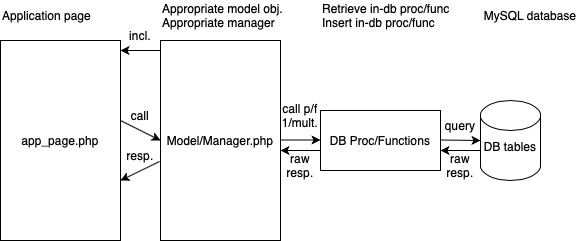
\includegraphics[scale=0.707]{img/app-schema.jpg}
\section{Managers}
Managers are written to provide API functionality for system administration in PHP. These managers are populating pages or taking new input from them and administer process of storing them. Each object has a manager handling it and accomodates database loads and stores controlled by transactions.
\begin{itemize}
    \item Post/PostsManager
    \item User/UsersManager
    \item Page/PagesManager
    \item Club/ClubsManager
    \item Cup/CupsManager
    \item Position/PositionsManager
    \item Region/RegionsManager
\end{itemize}
Managers are implemented to extract and store data of class by which they are named after. Let's take PostsManager as an example. This manager handles Post and is implemented as follows.
\newline
\textbf{Post.php}
\begin{lstlisting}
class Post
{
    public $id;
    public $timestamp;
    public $title;
    public $content;
    public $display_flag;
    public $author_user_id;
	public $signature_flag;

    public function __construct($id, $timestamp, $title, $content, $display_flag, $author_user_id, $signature_flag)

	//7/7: {id, timestamp, title, content, display_flag, author_user_id, signature_flag}
	public function Serialize()
}

\end{lstlisting}
\textbf{PostsManager.php} 
\begin{lstlisting}
class PostsManager
{
	private $mysqli;

    //Constructor - setting $mysqli to $this->mysqli
	public function __construct(mysqli $mysqli)

    //Handling functions retrieve/store  
	public function GetPostById($id)
  	public function FindLastNPosts($N)
	public function InsertNewPost($title, $content, $display_flag, $author, $signature_flag)
    public function UpdatePost($id, $title, $content, $display_flag, $signature_flag)

    //Private functions - auxiliary controller functions
	private function _CreatePostOrNullFromStatement(mysqli_stmt $statement)
	private function _CreatePostsFromStatement(mysqli_stmt $statement)
	private function _CreatePostFromRow(array $row)
}
\end{lstlisting}
\textbf{Demonstration - public function GetPostByID(\$id)}
\begin{lstlisting}
public function GetPostByID($id)
{
	$statement = $this->mysqli->prepare("CALL `GetPostByID`(?);");
	$statement->bind_param('i', $id);
	return $this->_CreatePostOrNullFromStatement($statement);
}
\end{lstlisting}
\section{Start file}
Start file is included the in beginning of each page. It serves for \textbf{connection to database},  \textbf{sanitization of input}, \textbf{definition of error handling} and most importantly \textbf{includes objects and managers} and subsequently \textbf{instantiates all managers} while passing reference to the database connection \textbf{\$mysqli} their only constructor argument.
\begin{lstlisting}
/*Database credentials from environment*/
$host = getenv("DATABASE_HOST");
$user = getenv("DATABASE_USER");
$pass = getenv("DATABASE_PASS");
$db   = getenv("DATABASE_NAME");
/*Database connection and charset set*/
$mysqli = new mysqli($host, $user, $pass, $db) or die($mysqli->error);
$mysqli->set_charset('utf8');
/* Sanitization function */
function h($string)
{
    return htmlspecialchars($string);
}
/* Exception handling*/
error_reporting(E_ALL);
ini_set("display_errors", 1);
set_exception_handler(function () {
    echo "<h3 style=\"color: red;\">INVALID REQUEST</h3>";
    exit();
});
/* Objects and Managers*/
require __DIR__ . '/model/Sanitizer.php';
require __DIR__ . '/model/Auth.php';
require __DIR__ . '/model/Post.php';
require __DIR__ . '/model/PostsManager.php';
require __DIR__ . '/model/Page.php';
require __DIR__ . '/model/PagesManager.php';
require __DIR__ . '/model/StatUserCnt.php';
require __DIR__ . '/model/StatPositionCnt.php';
require __DIR__ . '/model/RefereeRank.php';
require __DIR__ . '/model/Region.php';
require __DIR__ . '/model/RegionsManager.php';
require __DIR__ . '/model/User.php';
require __DIR__ . '/model/UsersManager.php';
require __DIR__ . '/model/Cup.php';
require __DIR__ . '/model/PairPositionUser.php';
require __DIR__ . '/model/CupsManager.php';
require __DIR__ . '/model/Position.php';
require __DIR__ . '/model/PositionsManager.php';
require __DIR__ . '/model/Club.php';
require __DIR__ . '/model/ClubsManager.php';
/* Construction of Managers w/ reference to $mysqli */
$postsManager     = new PostsManager($mysqli);
$pagesManager     = new PagesManager($mysqli);
$usersManager     = new UsersManager($mysqli);
$clubsManager     = new ClubsManager($mysqli);
$cupsManager      = new CupsManager($mysqli);
$positionsManager = new PositionsManager($mysqli);
$regionsManager = new RegionsManager($mysqli);
\end{lstlisting}
\section{Templating of web and administration}
Each page layout of public website has common characteristics such as header, menu and footer. These sections are unified and included everywhere, therfore they are included everywhere. They are:
\begin{itemize}
    \item HEADER,
    \item MENU,
    \item Generated from result obtained by one or more manager calls. this section might be further updated via XMLHttpRequest calls \& DOM modifications of newly delivered data,
    \item FOOTER.
\end{itemize}
Homepage of administration panel /admin/profile.php after login gets assembled with regards to the rights of logged user. Ordering is following: Admin (2) \textgreater \: Club manager (1) \textgreater \: Swimming referee (0) and each user gets snippet of his and lower role snippets:
\begin{itemize}
    \item SUPERUSER menu snippet - 2,
    \item CLUB MANAGER menu snippet - 1,
    \item SWIMMING REFEREE menu snippet - 0.
\end{itemize}
Following flow is then discriminated based on rights code on each page. \newline
\textbf{Rights check} 
\begin {lstlisting}
<?php
    require __DIR__ . '/../start.php';
    session_start();
    Auth::requireRole(UserRights::SuperUser);
    ...
?>    
...
\end{lstlisting}
\textbf{requireRole on Auth class} 
\begin{lstlisting}
class Auth
{
	public static function requireRole($role)
	{
		if (!isset($_SESSION['rights']))
        {
			header('Location: /prihlaseni.php');
			exit();
		}
		//Rights sharply lower that user has, throw RuntimeException
		if ($_SESSION['rights'] < $role)
        {
			echo '<h1>Not enough rights</h1>';
			echo $_SESSION['rights'];
			echo $role;
			throw new RuntimeException();
		}
	}
}
\end{lstlisting}
\section{Responsive layout}
Listed media queries are used to provide design of the web by manually overriding specific classes for desired user experience outcome.
\begin{itemize}
    \item Basic CSS design
    \item @media (max-width: 768px)
    \item @media (print)
\end{itemize}
\textbf{Basic CSS design} gives definition of colors and desktop layout of our application. \textbf{Media query with max-width: 768px} supports tablets and mobile devices while \textbf{media print} of cup pairing hides redundant controll and informative elements while it keeps the pairing of cup to be printed.
\section{Administrative tasks}
\begin{itemize}
    \item \textbf{Add Post/Edit Post} - from PostsManager call \newline InsertNewPost/UpdatePost
    \item \textbf{Approve Newly Registered Users} - swap flag \textbf{approved} to \textbf{1}
    \item \textbf{Pair Available Users On Cup Positions} - from UsersManager call UpdatePairing - calls several SQL Procs for different things in transaction and commits/rollbacks
    \item \textbf{Add User/Edit User} - from UsersManager call AddUser/UpdateUser
    \item \textbf{Add Cup/Edit Cup} - from CupsManager call AddCup/UpdateCup
    \item \textbf{Add Club/Edit Club} - from ClubsManager call AddClub/UpdateClub
    \item \textbf{Add Region/Edit Region} - from RegionsManager call AddRegion/UpdateRegion
    \item \textbf{Configure Stats Ordering} - delete ordering, insert ordering \textbf{Nth}-\textbf{statId} 
    \item \textbf{Edit Contacts} - from PagesManager call UpdatePage
\end{itemize} 
\section{Club Manager tasks}
\begin{itemize}
    \item \textbf{Add Cup} - from CupsManager call AddCup
    \item \textbf{Sign Up People From My Club As Available For Cup} - prihlasit\_moje\_lidi\_na.php then XMLHttpRequest/call\_update\_availability.php
\end{itemize}   
\section{Referee}    
\begin{itemize}
    \item \textbf{Sign Myself As Available For Cup} - add my Id to table \textbf{cupId}-\textbf{userId}
\end{itemize}